% Provenance (never printed): see sources/outline_sources.md (Year 2: palaeogeography through
% the Phanerozoic; sea level; orogenies; mass extinctions and their Earth causes). Maps from the
% plate model of Merdith and others (2021) through the GPlates Web Service; sea level from the
% Miller and others (2005) NOAA study (Haq and others 1987; Kominz and others 2008); flooding and
% the Pitman model after Tasistro-Hart and Macdonald (2023); the big five after Marshall (2023)
% and Kaiho (2022); oceanic anoxic events after Rigo and others (2024) and Walker-Trivett and
% others (2024); CAMP carbon dioxide after Capriolo and others (2020); Chicxulub after
% Pickersgill and others (2026) and Collins and others (2020). Curves and numbers from
% figdata/bachelor-2/phanerozoic.py; exercise and problem values in the Book 4 scratch
% calculator calc/ch19.py.
\chapter{显生宙的地球}\label{ch:b2:phanerozoic-earth}

在北美洲中部的堪萨斯州西部，一根根白色的白垩石柱
从草原上拔地而起。白垩是海底软泥的沉积：约 8000 万年前，一片
浅海自北向南横贯北美洲中部，漂浮藻类的
壳体以每年仅几百分之一毫米的速度落在其海底。在过去
5.4 亿年间，曾五次有大量生活于此类海洋中的物种在
一个地质瞬间内消亡。两段故事都是地球自身的历史：大陆漂移，海平面在其上升降，
而五次大灭绝中至少有三次，发生在来自地球内部的熔岩喷发之时。
本章沿显生宙的脉络，考察其古地图、海平面、\omterm{def:b2:alpine-orogen:orogen}{造山
带}与危机，并给出其中两例的数值：海岭如何抬升海平面，
以及海平面升高会淹没多少陆地。
% ledger: kgs:monument-rocks, kgs:chalk, ics:base.Phanerozoic, kaiho22:table, cr03:table

\begin{recall}
\textbf{来自中学阶段分册}：板块构造与泛大陆；化石与地质
年代表；在悬崖上读出的\omterm{def:b2:phanerozoic-earth:transgression}{海侵}。\textbf{来自本科一年级分册}：洋底的深度–年龄关系；
海陆起伏曲线；地壳均衡；全球海平面变化与相对海平面；大火成岩
省；作为地层标志的大灭绝，K--Pg 界线的铱，以及
二叠纪末危机的测年；阶与 GSSP。\textbf{来自前面各章}：\omterm{def:b2:alpine-orogen:orogen}{造山带}
（\cref{ch:b2:alpine-orogen,ch:b2:himalaya-andes}）；\omterm{def:b2:wilson-cycle:wilson}{威尔逊旋回}与\omterm{def:b2:wilson-cycle:supercontinent}{超大陆}
（\cref{ch:b2:wilson-cycle}）；\omterm{def:b2:basins-compared:backstripping}{回剥}（\cref{ch:b2:basins-compared}）；成冰纪
雪球事件（\cref{ch:b2:precambrian-earth}）。灭绝与生命史属于生物学分册；
本科三年级分册讨论古地磁学与层序地层学。
\end{recall}

\section{运动世界中的地图}\label{sec:b2:phanerozoic-earth:maps}

岩石很少仍在其形成的地方。煤、沙漠砂岩与礁：每一种都是在某个纬度
沉积下来的，此后便随所在板块一起迁移。要从这些岩石中读出过去某一时期的
气候或生命，必须先将它们放回原来的位置。

\begin{definition}[古地理学；古地理图]\label{def:b2:phanerozoic-earth:palaeogeography}
\emph{古地理学}\index{古地理学}是对过去某一
时期地理面貌的重建：大陆与海洋的位置，以及其海岸线、\omterm{def:b2:alpine-orogen:orogen}{造山带}与
海的分布。\emph{古地理图}\index{古地理图}显示某一时刻的该地理面貌，
底图采用该时刻的经纬网。
\end{definition}

此类地图依据四类证据绘制。岩石的磁化强度给出其形成时的纬度，
这是本科三年级分册古地磁学的主题；但地球磁场关于自转轴对称，
因此对经度毫无信息。洋底记录了板块的运动，
直接通过其磁条带与年龄，但只能追溯到
现存最老的洋底，约 1.9 亿年前；更老的洋底已俯冲殆尽。在此之前，
大陆拼合、洋盆闭合处的缝合带与\omterm{def:b2:alpine-orogen:orogen}{造山带}，以及
能够揭示气候的化石与沉积物——热带的礁与蒸发岩、
极地附近的冰川沉积——共同补全了图景。板块模型综合这些约束，将每块板块回溯到
过去某一刻的位置；重建还须考虑整个固体地球相对
其自转轴的缓慢转动，称为真极移。
% ledger: vh26:palaeogeography, gws:merdith-frame, data:b2-seafloor-age, merdith21:model

\begin{omfigure}
\centering
% figdata/bachelor-2/phanerozoic.py parts map-<t>, cities-<t>, grat (Mollweide, x and y in Earth radii)
\begin{tikzpicture}
\begin{groupplot}[group style={group size=2 by 3, horizontal sep=0.35cm, vertical sep=0.55cm},
  width=0.53\linewidth, axis equal image, hide axis, clip=false,
  xmin=-2.85, xmax=2.85, ymin=-1.43, ymax=1.43,
  title style={font=\small, yshift=-1.5ex}]
\pgfplotsinvokeforeach{500,300,200,100,50,0}{
\nextgroupplot[title={#1~\unit{Ma}}]
\fill[omSea] (axis cs:0,0) ellipse [x radius=2.8284, y radius=1.4142];
\addplot[fill=omLithAlluv!85!black, draw=none] table[x=x, y=y]
  {figdata/out/bachelor-2-phanerozoic-map-#1.dat};
\addplot[black!35, line width=0.2pt] table[x=x, y=y] {figdata/out/bachelor-2-phanerozoic-grat.dat};
\draw[black!70, line width=0.4pt] (axis cs:0,0) ellipse [x radius=2.8284, y radius=1.4142];
\addplot[only marks, mark=*, mark size=1.3pt, red!75!black, point meta=explicit symbolic,
  nodes near coords, nodes near coords style={font=\tiny\bfseries, anchor=south west,
  inner sep=0.5pt, text=red!60!black}]
  table[x=x, y=y, meta=tag] {figdata/out/bachelor-2-phanerozoic-cities-#1.dat};
}
\end{groupplot}
\end{tikzpicture}
\par\smallskip{\small 今日海岸线回溯到六个时刻，所用板块模型出自
Merdith 等（2021），由 GPlates Web Service 重建，采用等面积 Mollweide
投影；纬线每隔 \ang{30} 一条，经线每隔 \ang{60} 一条。红点标示四座城市：
巴黎（P）、纽约（N）、悉尼（S）与开普敦（C）；在 \qty{500}{Ma} 时，
悉尼所在的地壳尚未进入模型。图中形状是今日海岸线经移动后的结果，并非
当时的海岸线；在这一古地磁参照系中，经度是任意的。}
\end{omfigure}
% ledger: data:b4-palaeocoast, data:b4-palaeopos, geonames4:cities, gws:merdith-frame, merdith21:model

上面六幅图概括了显生宙。在 \qty{500}{Ma} 时，南方诸大陆连成一片，
即冈瓦纳大陆，大部分靠近南极，巴黎所在地壳位于其
边缘，南纬 \ang{61}。到 \qty{300}{Ma} 时，各大陆已拼合为泛大陆，
拼合始于约 \qty{325}{Ma}，裂解始于约 \qty{200}{Ma}：巴黎与纽约位于赤道上，开普敦
与悉尼位于 南纬 \ang{60} 附近。在 \qty{200}{Ma} 时，\omterm{def:b2:wilson-cycle:supercontinent}{超大陆}已完整形成，
是一块从北高纬延伸到南高纬的陆地；到 \qty{100}{Ma} 时，大西洋与印度洋已张开，
到 \qty{50}{Ma} 时，地图已与今日相近，澳大利亚仍靠近南极洲。
% ledger: data:b4-palaeopos, nance22:supercontinents

\begin{example}[巴黎向北漂移]\label{ex:b2:phanerozoic-earth:paris}
在该模型中，巴黎在 \qty{300}{Ma} 前位于 北纬 \ang{5.1}，今日位于 北纬 \ang{48.9}。其
纬度增加了 \ang{43.8}，即沿经线距离 $43.8 \times 111.2 = \qty{4871}{km}$
（球面半径取 \qty{6371}{km}，每度对应 $\qty{111.2}{km}$），平均速率为
$4871/300 = \qty{16}{km}$ 每百万年，或每年 \qty{1.6}{cm}。这只是
向北运动的部分：古地磁参照系对经度不加约束，因此实际
行进距离至少不小于此值。
\end{example}
% ledger: data:b4-palaeopos, geonames4:cities, earth:Rmean, gws:merdith-frame
% values: calc/ch19.py (43.8 deg, 4870.6 km, 16.2 km/Myr)

\section{显生宙的海平面}\label{sec:b2:phanerozoic-earth:sealevel}

\subsection*{大陆上的海}

在显生宙的大部分时间里，大陆被海水覆盖的范围远大于今天。北美
的海相岩层记录了大陆内部的数次淹没，其中最早的一次是
寒武纪\omterm{def:b2:phanerozoic-earth:transgression}{海侵}，它封存了大不整合；在晚白垩世，
约 120 至 \qty{80}{Ma} 期间，海相沉积物横跨西部内陆，
位于大陆中部（见下图）。
% ledger: th23:flooding, th23:wib

\begin{omfigure}
\centering
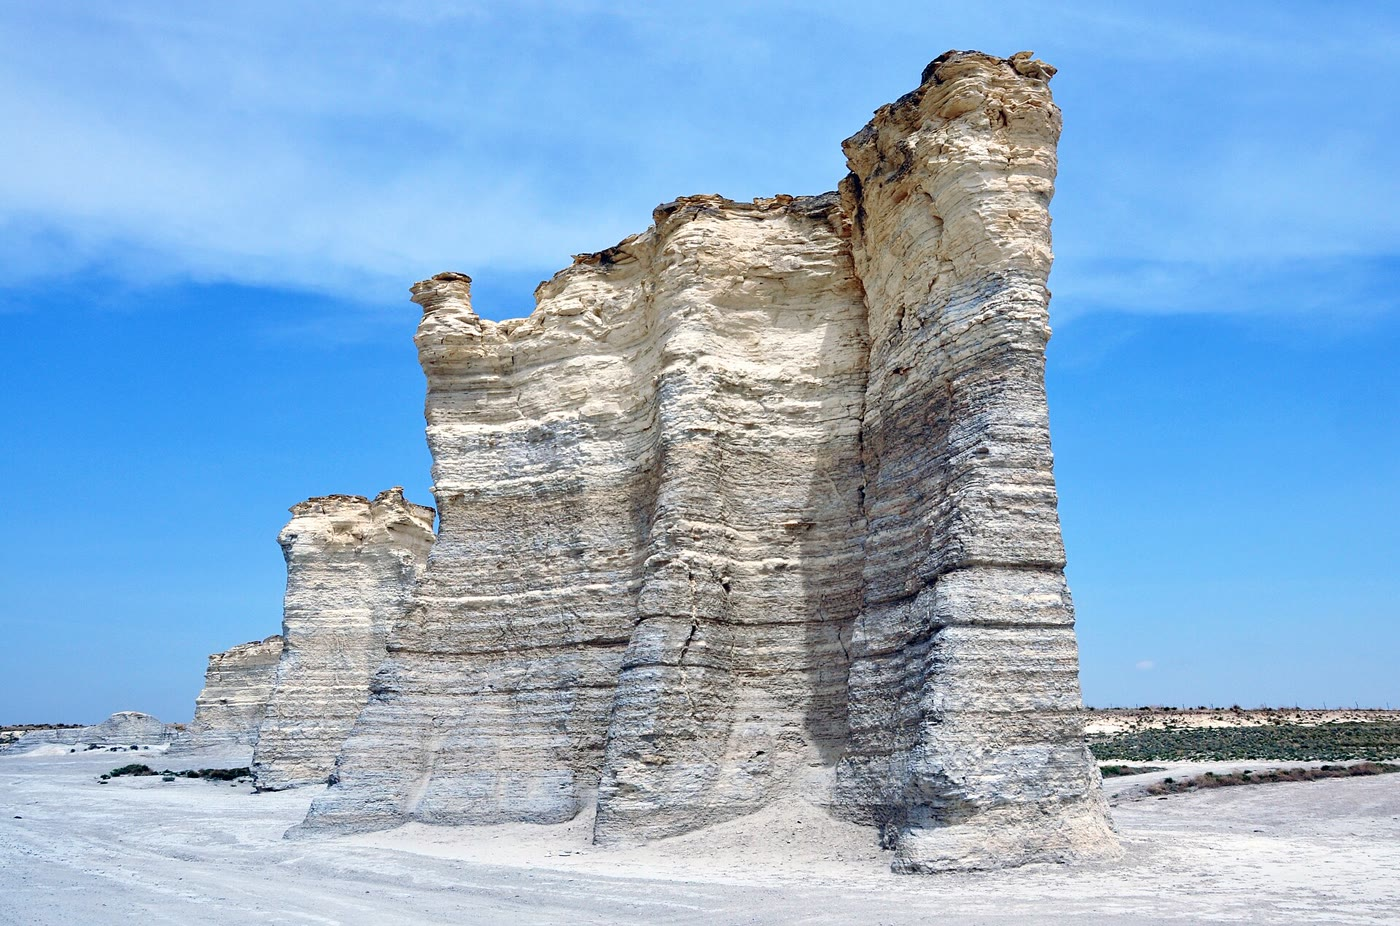
\includegraphics[width=0.66\linewidth]{images/book4/b2-19-monument-rocks.jpg}
\par\smallskip{\small 堪萨斯州西部的 Monument Rocks：白垩岩柱，是一片约 8000 万年前的白垩纪
内陆海留下的软泥沉积，沉积速率约为每年 \qty{0.036}{mm}。（James
St.~John，CC~BY~2.0，经维基共享资源。）}
\end{omfigure}
% ledger: kgs:monument-rocks, kgs:chalk

\begin{definition}[陆表海]\label{def:b2:phanerozoic-earth:epeiric}
称\emph{陆表海}\index{陆表海}为一种浅海，它漫布于大陆内部，
位于大陆地壳之上，远离大陆边缘。
\end{definition}

海水通过移动岸线抵达这类大陆内部，岩层记录了这一移动。

\begin{definition}[海侵；海退]\label{def:b2:phanerozoic-earth:transgression}
称\emph{海侵}\index{海侵}为岸线向陆地方向的移动，
海水由此漫过陆地；称\emph{海退}\index{海退}为
岸线向海方向的移动，陆地由此露出。
\end{definition}

在竖直剖面中，\omterm{def:b2:phanerozoic-earth:transgression}{海侵}使较深水沉积叠在较浅水沉积之上——
离岸泥覆于海滩砂之上——\omterm{def:b2:phanerozoic-earth:transgression}{海退}则相反。两者都受相对
海平面控制，它综合了全球海平面、当地沉降或抬升，以及沉积物
的供给；若供给足够快，三角洲在海面上升时仍可将岸线推向海方向。
要从\omterm{def:b2:phanerozoic-earth:transgression}{海侵}中读出全球海平面，地质学家必须在数个大陆上找到相同的信号，
或通过\omterm{def:b2:basins-compared:backstripping}{回剥}法去除沉降的影响（
见\cref{ch:b2:basins-compared}）。
% ledger: miller20:rsl

\subsection*{长期曲线}

\begin{definition}[一级海平面旋回]\label{def:b2:phanerozoic-earth:first-order}
称\emph{一级海平面旋回}\index{一级海平面旋回}为全球海平面变化中
最慢的部分，时间尺度为数千万至数亿年，
由固体地球的构造作用决定，而非由冰决定。
\end{definition}

在整个显生宙中，一级曲线呈 M 形：早古生代海平面高，
泛大陆聚合并存续期间（自石炭纪至三叠纪末）海平面低，
白垩纪再次升高，此后持续下降。由北美推断，仅晚奥陶世的
淹没一项，就提示海平面还应再高出 100 至 \qty{200}{m}。
更快的变化叠加在这条曲线之上：由冰驱动的变化记录于 $10^4$ 至
$10^6$ 年的时间尺度上，南极冰盖自约 \qty{33.5}{Ma} 起使海平面变化了 50 至
\qty{60}{m}。
% ledger: th23:flooding, miller11:greenhouse, miller05:abstract

\begin{omfigure}
\centering
% figdata/bachelor-2/phanerozoic.py parts sealevel-haq, sealevel-haqlt, sealevel-kominz, sealevel-kominzlt
\begin{tikzpicture}
\begin{axis}[width=0.92\linewidth, height=6.2cm, x dir=reverse, xmin=0, xmax=252,
  ymin=-130, ymax=280, xlabel={年龄（\unit{Ma}）}, ylabel={海平面高于今日（\unit{m}）},
  xtick={0,50,...,250}, ytick={-100,-50,...,250}, xtick pos=bottom, ytick pos=left,
  tick label style={font=\scriptsize}, label style={font=\small},
  legend style={at={(0.5,1.04)}, anchor=south, draw=none, font=\scriptsize, legend columns=2,
  /tikz/every even column/.append style={column sep=8pt}}]
\addplot[black!30, line width=0.3pt] table[x=age_ma, y=sl_m]
  {figdata/out/bachelor-2-phanerozoic-sealevel-haq.dat};
\addlegendentry{Haq 等（1987）}
\addplot[omThm, line width=0.3pt] table[x=age_ma, y=sl_m]
  {figdata/out/bachelor-2-phanerozoic-sealevel-kominz.dat};
\addlegendentry{新泽西，回剥}
\addplot[black, line width=1.2pt] table[x=age_ma, y=sl_m]
  {figdata/out/bachelor-2-phanerozoic-sealevel-haqlt.dat};
\addlegendentry{Haq，10-Ma 均值}
\addplot[omThm!70!black, line width=1.2pt] table[x=age_ma, y=sl_m]
  {figdata/out/bachelor-2-phanerozoic-sealevel-kominzlt.dat};
\addlegendentry{新泽西，10-Ma 均值}
\addplot[black!50, line width=0.3pt, forget plot] coordinates {(0,0) (252,0)};
\foreach \a/\b/\c in {251.902/201.4/icsTriassic, 201.4/143.1/icsJurassic,
  143.1/66/icsCretaceous, 66/23.04/icsPaleogene, 23.04/2.58/icsNeogene, 2.58/0/icsQuaternary} {
  \edef\tmp{\noexpand\fill[\c] (axis cs:\a,-130) rectangle (axis cs:\b,-112);}\tmp}
\node[font=\tiny, text=white] at (axis cs:226.7,-121) {三叠纪};
\node[font=\tiny, text=white] at (axis cs:172.3,-121) {侏罗纪};
\node[font=\tiny] at (axis cs:104.6,-121) {白垩纪};
\node[font=\tiny] at (axis cs:44.5,-121) {古近纪};
\node[font=\tiny] at (axis cs:12.8,-121) {新近纪};
\end{axis}
\end{tikzpicture}
\par\smallskip{\small 自 \qty{250}{Ma} 以来的全球海平面，据 Miller 等（2005）整理：
一是 Haq 等（1987）根据众多盆地地层绘制的旋回图，
二是新泽西岩芯\omterm{def:b2:basins-compared:backstripping}{回剥}所得的海平面，并标出估计的低水位期（Kominz 等，2008）。
粗线为 10-Ma 滑动平均，代表一级趋势。年龄依据
2012 年时间尺度；底部色条表示各纪。}
\end{omfigure}
% ledger: data:b4-sealevel, haq87:charts, kominz08:long-term, ics:base.Triassic, ics:base.Jurassic, ics:base.Cretaceous, ics:base.Paleogene, ics:base.Neogene, ics:base.Quaternary, ics:colour.Triassic, ics:colour.Jurassic, ics:colour.Cretaceous, ics:colour.Paleogene, ics:colour.Neogene, ics:colour.Quaternary

上面两条曲线形状一致，幅度却不相符。旋回图由
众多盆地沉积物的叠加构建，给出白垩纪中期的长期海平面
约高出今日 \qty{233}{m}；新泽西的钻井经逐一\omterm{def:b2:basins-compared:backstripping}{回剥}，给出晚白垩世约
\qty{70}{m}，始新世的最大值接近 \qty{110}{m}。Miller 及其
同事认为白垩纪长期峰值为 $100 \pm \qty{50}{m}$，并认为
旋回图对下降的时间判断正确，却夸大了其振幅。即便是新泽西，
也并非完美的指标：其晚白垩世的海面比大洋盆地的体积所预测的
低 100 至 \qty{150}{m}，这一差距可由俯冲的法拉隆板块之上
该区域的下沉——动力地形——来解释。
% ledger: data:b4-sealevel, miller05:abstract, kominz08:long-term, miller20:epr

\subsection*{海平面为何变动：洋脊}

什么能让海平面在数千万年间抬高 100 米？不是冰：白垩纪
是一个温暖的世界，至多只有小型、短暂的冰盖。主流的解释是洋脊的
体积。年轻洋底温度高、位置也高；板块扩张越快，
洋底平均越年轻，洋盆越浅，
溢到大陆上的海水也就越多。
% ledger: miller11:greenhouse, th23:pitman

\begin{proposition}[海平面与扩张速率]\label{prop:b2:phanerozoic-earth:ridge}
设面积为 $A_{\text{f}}$ 的洋底由总长为 $L$ 的洋脊以全
扩张速率 $u$ 生成，并在年龄 $\tau = A_{\text{f}}/(Lu)$ 时消亡，年龄介于 0
与 $\tau$ 之间的每一段洋底所占面积相同。设其深度服从规律 $d(t) = d_{\text{r}} + c\sqrt t$。
\begin{enumerate}
  \item 洋底的平均深度为 $\bar d = d_{\text{r}} + \tfrac23 c\sqrt\tau$。
  \item 若扩张速率变为 $fu$，而 $A_{\text{f}}$ 与 $L$ 不变，则平均
        深度减小 $\Delta\bar d = \tfrac23 c\sqrt\tau\,\bigl(1 - f^{-1/2}\bigr)$。
  \item 若洋底在所增加的海水负荷下发生均衡下沉，且海水不漫溢到陆地上，
        则面积为 $A_{\text{o}}$ 的海洋上的海平面上升
        \[
        \Delta s = \frac{\rho_{\text{m}} - \rho_{\text{w}}}{\rho_{\text{m}}}\,
        \frac{A_{\text{f}}}{A_{\text{o}}}\,\Delta\bar d ,
        \]
        其中 $\rho_{\text{m}}$ 为地幔密度，$\rho_{\text{w}}$ 为海水密度。
\end{enumerate}
\end{proposition}

\begin{proof}
(1) 洋脊以速率 $Lu$（单位时间的面积）生成新洋底，每一条洋底带的寿命都是
$\tau$；在稳态下，年龄介于 $t$ 与 $t + \mathrm{d}t$ 之间的洋底面积为
 $Lu\,\mathrm{d}t$（对所有 $t < \tau$），因此总面积为 $Lu\tau = A_{\text{f}}$，且
各年龄段分布均匀。平均深度为
$\frac1\tau\int_0^\tau (d_{\text{r}} + c\sqrt t)\,\mathrm{d}t = d_{\text{r}} + \frac{c}{\tau}
\cdot\frac23\tau^{3/2}$。(2) 扩张速率为 $fu$ 时，$\tau$ 变为 $\tau/f$，且
$\sqrt{\tau/f} = f^{-1/2}\sqrt\tau$。(3) 盆地损失的体积为 $\Delta V = A_{\text{f}}
\Delta\bar d$。设海面相对大陆上升 $\Delta s$，洋底
在额外海水负荷下下沉 $y$。额外的水柱厚 $\Delta s + y$，在均衡中替代了
厚度为 $y$ 的地幔：$\rho_{\text{w}}(\Delta s + y) =
\rho_{\text{m}} y$，故 $y = \rho_{\text{w}}\Delta s/(\rho_{\text{m}} - \rho_{\text{w}})$，且
$\Delta s + y = \Delta s\,\rho_{\text{m}}/(\rho_{\text{m}} - \rho_{\text{w}})$。体积
守恒：$A_{\text{o}}(\Delta s + y) = \Delta V$，由此得到结果。
\end{proof}

真实的洋底并不这么规整。其年龄分布并不均匀：年轻洋底所占面积最大，
面积随年龄增大而减小，如下方左图所示。对老洋底，平方根律也不再成立，
它在约 \qty{6.4}{km} 处趋于平缓；帕森斯与斯克莱特为老洋底拟合的指数律，
即板块律，在约 \qty{26}{Ma} 以后接替，两者在此
相交。本命题只是初步估计，下图
展示了第二种规律对其结果的改变有多大。
% ledger: ps77:depth-age, data:b4-ridge

\begin{omfigure}
\centering
% figdata/bachelor-2/phanerozoic.py parts agehist and ridge
\begin{tikzpicture}
\begin{groupplot}[group style={group size=2 by 1, horizontal sep=1.6cm},
  width=0.5\linewidth, height=5.6cm, tick label style={font=\scriptsize},
  label style={font=\small}, xtick pos=bottom, ytick pos=left]
\nextgroupplot[xmin=0, xmax=200, ymin=0, ymax=34, xlabel={洋底年龄 (\unit{Ma})},
  ylabel={每 \qty{10}{Ma} 的面积 (\unit{\mega km^2})},
  legend style={at={(0.5,1.04)}, anchor=south, draw=none, font=\scriptsize}]
\addplot[ybar interval, area legend, fill=omSea!80!black, draw=black!50, line width=0.2pt]
  table[x expr=\thisrow{age}-5, y=area_Mkm2] {figdata/out/bachelor-2-phanerozoic-agehist.dat};
\addlegendentry{年龄网格}
\addplot[const plot mark mid, black, dashed, line width=0.9pt]
  table[x=age, y=uniform_Mkm2] {figdata/out/bachelor-2-phanerozoic-agehist.dat};
\addlegendentry{年龄均匀分布至 \qty{128.4}{Ma}}
\nextgroupplot[xmin=1, xmax=3, ymin=0, ymax=650, xlabel={扩张速率 / 今日值，$f$},
  ylabel={海平面上升 $\Delta s$ (\unit{m})},
  legend style={at={(0.5,1.04)}, anchor=south, draw=none, font=\scriptsize, legend columns=2}]
\fill[omThm!15] (axis cs:1,50) rectangle (axis cs:3,150);
\addplot[black, line width=1pt] table[x=f, y=ds_hs] {figdata/out/bachelor-2-phanerozoic-ridge.dat};
\addlegendentry{$\sqrt t$ 律}
\addplot[blue!70!black, dashed, line width=1pt] table[x=f, y=ds_plate]
  {figdata/out/bachelor-2-phanerozoic-ridge.dat};
\addlegendentry{板块律}
\node[font=\scriptsize, anchor=west] at (axis cs:1.6,100) {$100 \pm \qty{50}{m}$};
\end{groupplot}
\end{tikzpicture}
\par\smallskip{\small 左图：今日洋底按 10-Ma 年龄区间统计的面积，取自塞顿等人（2020）的年龄网格
（一度分辨率，共 \qty{293}{\mega km^2}），与\cref{prop:b2:phanerozoic-earth:ridge}中的
面积与平均年龄相同的年龄均匀分布相比较。右图：
扩张速率乘以 $f$ 时的海平面上升，由命题在
平方根律与板块律下计算，从年龄均匀分布起算，直至 \qty{128.4}{Ma}；
色带为米勒等人（2005）估计的白垩纪长期峰值。}
\end{omfigure}
% ledger: data:b4-ridge, data:b2-seafloor-age, seton:mean-age, ps77:depth-age, miller05:abstract, charette:ocean-volume, katz03:thermo, noaa:seawater-1025

\begin{example}[速率翻倍]\label{ex:b2:phanerozoic-earth:doubling}
取今日的洋底：平均年龄 \qty{64.2}{Ma}，故在均匀分布模型中 $\tau = \qty{128.4}{Ma}$；
$d_{\text{r}} = \qty{2500}{m}$，$c = \qty{350}{m.Ma^{-1/2}}$。平均深度为 $2500 + \tfrac23
\times 350 \times \sqrt{128.4} = \qty{5144}{m}$。速率加倍使 $\tau$ 减半，平均
深度变为 $2500 + \tfrac23 \times 350 \times \sqrt{64.2} = \qty{4370}{m}$，即洋底平均
上升 \qty{774}{m}。取 $A_{\text{f}}/A_{\text{o}} = 293/362 = 0.8094$，且
$(\rho_{\text{m}} - \rho_{\text{w}})/\rho_{\text{m}} = (3300 - 1025)/3300 = 0.689$，则海平面上升
$0.689 \times 0.8094 \times 774 = \qty{432}{m}$；按板块律则为 \qty{368}{m}。两者均约为
白垩纪长期峰值的四倍左右。反过来看，右图表明，
仅比今日高 15 至 \qty{20}{\percent} 的扩张速率，便足以产生 \qty{100}{m} 的上升——这正是
米勒及其同事作出如下结论的原因：白垩纪洋壳的生成速度远慢于
此前所推断。
\end{example}
% ledger: seton:mean-age, ps77:depth-age, data:b4-ridge, charette:ocean-volume, katz03:thermo, noaa:seawater-1025, miller05:abstract
% values (phanerozoic.py numbers): dbar_hs 5144, dbar_hs_half 4369.6, rise2_hs 432.5, rise2_pl 368.4, f_for_100_hs 1.151

模型也偏深：其平均深度 \qty{5144}{m} 超过了定年洋底的实测平均深度
\qty{4265}{m}，部分是由于平方根律在老洋底上估计过高，且
部分是由于真实洋底还带有沉积物、\omterm{def:b2:oceanic-islands:seamount}{海山}与海底高原，这些都是该律所未包含的。扩张速率并非
唯一的杠杆。洋脊由海沟平衡：若某处洋底抬升，其质量必然
去往别处，而板片之上的大陆下沉——动力地形——使海水得以
局部侵入。塔西斯特罗-哈特与麦克唐纳认为，北美的洪泛随大陆之下的板片
而发生，并认为全球海平面取决于俯冲有多少发生在大陆之下，
而非大洋之下。
% ledger: data:b4-floor-depth, th23:pitman, th23:flooding, kominz08:long-term

\section{淹没大陆}\label{sec:b2:phanerozoic-earth:flooding}

海面上升会淹没多少陆地，取决于地表的形状，这一形状由
本科一年级分册中的海陆起伏曲线给出：地表中高于各个高程的部分所占比例
（见下图左）。大陆顶部较为平坦。ETOPO1 的一度网格显示，
陆地占地表的 \qty{29.0}{\percent}，而高于
\qty{-200}{m} 的部分占 \qty{34.3}{\percent}：大陆架本已在水下，两者之差正在于此。大部分陆地地势低，因此
海面小幅上升便会淹没其中相当大的一部分。
% ledger: data:b4-hyps, data:etopo1

\begin{proposition}[陆地的淹没]\label{prop:b2:phanerozoic-earth:flooding}
设 $A_{\text{o}}$ 为今日海洋的面积，$a(z)$ 为今日海平面以上
高度低于 $z$ 的陆地面积。向海洋加入体积为 $V$ 的水后，海面升高的高度 $s$
满足
\[
V = \int_0^s \bigl(A_{\text{o}} + a(z)\bigr)\,\mathrm{d}z ,
\]
并淹没面积为 $a(s)$ 的陆地。由于 $a \ge 0$，海面升高至多为 $V/A_{\text{o}}$。
\end{proposition}

\begin{proof}
海面位于 $z$ 时覆盖面积 $A_{\text{o}} + a(z)$，将其升高 $\mathrm{d}z$ 所需的
水量为 $\bigl(A_{\text{o}} + a(z)\bigr)\mathrm{d}z$。从 0 到 $s$ 积分得 $V$。被积函数
不小于 $A_{\text{o}}$，因此 $V \ge A_{\text{o}}s$。
\end{proof}

\begin{omfigure}
\centering
% figdata/bachelor-2/phanerozoic.py parts hyps and flood
\begin{tikzpicture}
\begin{groupplot}[group style={group size=2 by 1, horizontal sep=1.6cm},
  width=0.46\linewidth, height=5.6cm, tick label style={font=\scriptsize},
  label style={font=\small}, xtick pos=bottom, ytick pos=left]
\nextgroupplot[xmin=0, xmax=100, ymin=-9500, ymax=6500,
  xlabel={高于 $z$ 的地表百分比}, ylabel={高程 $z$（\unit{m}）},
  scaled y ticks=false, yticklabel style={/pgf/number format/1000 sep={\,}}]
\addplot[omThm, line width=1pt] table[x=pct, y=z] {figdata/out/bachelor-2-phanerozoic-hyps.dat};
\addplot[black!50, line width=0.3pt] coordinates {(0,0) (100,0)};
\node[font=\scriptsize, anchor=south west] at (axis cs:30,100) {陆地 \qty{29.0}{\percent}};
\node[font=\scriptsize] at (axis cs:45,-7000) {洋底};
\nextgroupplot[xmin=0, xmax=1000, ymin=0, ymax=80, xlabel={海平面上升 $h$（\unit{m}）},
  ylabel={被淹没的陆地（\unit{\percent}）}]
\addplot[omThm, line width=1pt] table[x=h, y=flooded_pct]
  {figdata/out/bachelor-2-phanerozoic-flood.dat};
\addplot[black, dashed, line width=0.5pt] coordinates {(100,0) (100,14.9) (0,14.9)};
\addplot[black, dashed, line width=0.5pt] coordinates {(432,0) (432,50.6) (0,50.6)};
\end{groupplot}
\end{tikzpicture}
\par\smallskip{\small 左：来自 ETOPO1 一度网格的地球海陆起伏曲线。
右：今日陆地中低于海平面以上各高程的百分比，即若其他条件不变，海面上升 $h$ 所淹没的陆地；
虚线标出 \qty{100}{m} 与 \qty{432}{m}。对一度格元取平均会平滑地形起伏，
因此这些只是初步估计。}
\end{omfigure}
% ledger: data:b4-hyps, data:etopo1

右图可立即给出答案：海面上升 \qty{100}{m} 可淹没约
\qty{15}{\percent} 的今日陆地；扩张速率加倍所对应的 \qty{432}{m} 则会淹没一半。
这样的海水会铺展于其所淹没的陆地之上，因此海面升高本身
小于命题中的上界 $V/A_{\text{o}}$，对几百米的上升约小一成（
周末问题）。白垩纪时堪萨斯的海所需的海面上升要小得多：大陆内部常常
地势低平，它也可能随板片而下沉。
% ledger: data:b4-hyps
% values (phanerozoic.py numbers): flood_100 14.9, flood_rise2 50.8, level_rise2_spread 390.7

\section{显生宙的造山带}\label{sec:b2:phanerozoic-earth:orogens}

\cref{ch:b2:wilson-cycle}中的每个\omterm{def:b2:wilson-cycle:wilson}{威尔逊旋回}都止于一条\omterm{def:b2:alpine-orogen:orogen}{造山带}，显生宙的
\omterm{def:b2:alpine-orogen:orogen}{造山带}记录了泛大陆的形成与破裂。下表汇集了本分册中出现过的各\omterm{def:b2:alpine-orogen:orogen}{造山带}。

\begin{center}
\small
\begin{tabular}{>{\raggedright\arraybackslash}p{0.15\linewidth}>{\raggedright\arraybackslash}p{0.22\linewidth}>{\raggedright\arraybackslash}p{0.22\linewidth}>{\raggedright\arraybackslash}p{0.29\linewidth}}
\hline
造山作用 & 时间 & 闭合的洋 & 相遇的陆块 \\
\hline
加里东 & 约 540--400 Ma；主碰撞 425--400 Ma & 伊阿珀托斯洋 & 劳伦古陆、波罗的古陆与
阿瓦隆古陆，形成劳亚古陆 \\
瓦里斯坎–阿巴拉契亚 & 始于约 550 Ma；最终碰撞于晚石炭世–二叠纪 & 雷克洋 &
冈瓦纳古陆及其分离出的\omterm{def:b2:wilson-cycle:terrane}{地体}与劳亚古陆相碰，形成泛大陆 \\
阿尔卑斯 & 白垩纪（峰值约 100 Ma）及新生代 & 阿尔卑斯特提斯洋 & 阿普利亚与欧洲 \\
喜马拉雅 & 约 60 至 54 Ma（有争议）起至今 & 印度以北的洋 & 印度与亚洲 \\
安第斯 & 仍在活动；自渐新世起持续缩短 & 无：一块洋板块俯冲 & 纳斯卡
板块位于南美洲之下 \\
\hline
\end{tabular}
\end{center}
% ledger: mckerrow00:caledonian, schiffer20:caledonides, schiffer20:variscan, faure24:variscan, usgs:alleghanian-age, schmid04:two-orogenies, najman21:collision-age, gerbault05:andes, nance22:supercontinents

前两条\omterm{def:b2:alpine-orogen:orogen}{造山带}将泛大陆缝合在一起，其中瓦里斯坎\omterm{def:b2:alpine-orogen:orogen}{造山带}闭合了冈瓦纳古陆与
劳亚古陆之间最后的洋；后三条随泛大陆各块彼此分开而生长，其间的洋
被消耗殆尽。晚古生代与三叠纪的低海平面属于这一
\omterm{def:b2:wilson-cycle:supercontinent}{超大陆}，白垩纪的高海平面则对应其破裂，伴随新的洋脊与年轻的
洋底。
% ledger: schiffer20:variscan, th23:flooding, nance22:supercontinents

\section{生命危机}\label{sec:b2:phanerozoic-earth:extinctions}

\subsection*{五大灭绝}

生物学分册描述了大灭绝；地质学家则在岩石中测量它们，并探寻
其成因。海洋动物的记录中有五次尤为突出，即“五大灭绝”：奥陶纪末，约
\qty{444}{Ma}；晚泥盆世，\qty{372}{Ma}；二叠纪末，
\qty{251.9}{Ma}；三叠纪末，\qty{201.4}{Ma}；以及白垩纪末，
\qty{66}{Ma}。按塞普科斯基的汇编，每次都使海洋动物的
属减少约五分之二至三分之二。二叠纪末的危机最大：在最精细的分辨率下，\qty{56}{\percent} 的
属，以及约 \qty{81}{\percent} 的海洋物种——并非
常被引用的 \qty{96}{\percent}，该数字混淆了两次彼此独立的危机。
% ledger: kaiho22:table, marshall23:big-five, stanley16:permian

\begin{history}[五大灭绝，四十年后]
1982 年，劳普与塞普科斯基统计了海洋动物中消失的科数，统计范围为
显生宙的 76 个阶中每一阶的情况。四个点高于其趋势的 99\% 置信限——
奥陶纪的最后一阶、二叠纪的最后两阶与白垩纪的
最后一阶——以及三叠纪末与泥盆纪末高于 95\%
置信限：即五大灭绝。四十年后，这五次仍是早奥陶世以来最大的几次危机，
但有了更好的数据后，它们不再从灭绝速率的连续谱中凸显出来，
寒武纪的某些时段灭绝速率甚至更高。劳普与塞普科斯基的时间
分辨率为 \qty{7.4}{Ma}，即当时阶的平均长度；有些危机突然发生，另一些
持续了数十万年或更久。
\end{history}
% ledger: marshall23:big-five, marshall23:resolution

\begin{omfigure}
\centering
% figdata/bachelor-2/phanerozoic.py parts ext, lip, oae
\begin{tikzpicture}
\begin{axis}[width=0.95\linewidth, height=6.4cm, x dir=reverse, xmin=0, xmax=541,
  ymin=-34, ymax=80, xlabel={年龄 (\unit{Ma})}, ylabel={消失的海洋属比例 (\unit{\percent})},
  xtick={0,100,...,500}, ytick={0,20,...,80}, xtick pos=bottom, ytick pos=left,
  tick label style={font=\scriptsize}, label style={font=\small}, clip=false]
\addplot[ybar, bar width=5pt, fill=omThm!70, draw=black!60, point meta=explicit symbolic]
  table[x=age, y=value, meta=label] {figdata/out/bachelor-2-phanerozoic-ext.dat};
\node[font=\tiny, anchor=south] at (axis cs:444,52) {奥陶纪末};
\node[font=\tiny, anchor=south] at (axis cs:372,41) {晚泥盆世};
\node[font=\tiny, anchor=south] at (axis cs:251.9,66) {二叠纪末};
\node[font=\tiny, anchor=south] at (axis cs:201.4,46) {三叠纪末};
\node[font=\tiny, anchor=south] at (axis cs:66,45) {白垩纪末};
\addplot[only marks, mark=triangle*, mark size=2.6pt, red!70!black]
  table[x=age, y expr=-6] {figdata/out/bachelor-2-phanerozoic-lip.dat};
\addplot[only marks, mark=diamond*, mark size=2.6pt, blue!70!black]
  table[x=age, y expr=-13] {figdata/out/bachelor-2-phanerozoic-oae.dat};
\addplot[only marks, mark=star, mark size=4pt, line width=1pt, black] coordinates {(66,-20)};
\node[font=\tiny, anchor=west, red!70!black] at (axis cs:541,-6) {大火成岩省};
\node[font=\tiny, anchor=west, blue!70!black] at (axis cs:541,-13) {大洋缺氧事件};
\node[font=\tiny, anchor=west] at (axis cs:541,-20) {撞击};
\node[font=\tiny, anchor=west] at (axis cs:57,-20) {希克苏鲁伯};
\foreach \a/\b/\c in {538.8/486.85/icsCambrian, 486.85/443.1/icsOrdovician,
  443.1/419.62/icsSilurian, 419.62/358.86/icsDevonian, 358.86/298.9/icsCarboniferous,
  298.9/251.902/icsPermian, 251.902/201.4/icsTriassic, 201.4/143.1/icsJurassic,
  143.1/66/icsCretaceous, 66/23.04/icsPaleogene, 23.04/2.58/icsNeogene, 2.58/0/icsQuaternary} {
  \edef\tmp{\noexpand\fill[\c] (axis cs:\a,-34) rectangle (axis cs:\b,-27);}\tmp}
\foreach \x/\t in {512.8/Cm, 465/O, 431.4/S, 389.2/D, 328.9/C, 275.4/P, 226.7/Tr, 172.3/J,
  104.6/K, 44.5/Pg, 12.8/N} {
  \edef\tmp{\noexpand\node[font=\noexpand\tiny] at (axis cs:\x,-30.5) {\t};}\tmp}
\end{axis}
\end{tikzpicture}
\par\smallskip{\small 显生宙五次大灭绝，海洋属消失比例取自
塞普科斯基汇编（Kaiho 2022，表~1）、大火成岩省（三角形，平均年龄据
Courtillot 与 Renne 2003，自 \qty{259}{Ma} 起算）、研究最充分的\omterm{def:b2:phanerozoic-earth:oae}{大洋缺氧事件}
（菱形）以及希克苏鲁伯撞击。底部的条带标出各纪。}
\end{omfigure}
% ledger: kaiho22:table, cr03:table, rigo24:oaes, pickersgill26:chicxulub, ics:base.Cambrian, ics:base.Ordovician, ics:base.Silurian, ics:base.Devonian, ics:base.Carboniferous, ics:base.Permian, ics:base.Triassic, ics:base.Jurassic, ics:base.Cretaceous, ics:base.Paleogene, ics:base.Neogene, ics:base.Quaternary, ics:colour.Cambrian, ics:colour.Ordovician, ics:colour.Silurian, ics:colour.Devonian, ics:colour.Carboniferous, ics:colour.Permian

\subsection*{大火成岩省}

上图显示了本科一年级分册所指出的规律：五次大灭绝中最近的三次，
各自都落在一个大火成岩省上：二叠纪末的西伯利亚暗色岩，
三叠纪末的中大西洋\omterm{def:b2:magma-emplacement:magma}{岩浆}省（CAMP），白垩纪末的德干暗色岩。
所提出的联系在于气体。一次溢流玄武岩以数百年至数千年为单位分脉冲喷发，
每一脉冲释放二氧化碳的速度超过风化作用回收的速度；
同一次喷发中的硫使气候短暂降温，
碳则使其长期增温，并使海洋酸化。
% ledger: cr03:table, cr03:summary, capriolo20:camp-co2

\begin{example}[中大西洋岩浆省的碳]\label{ex:b2:phanerozoic-earth:camp}
CAMP 玄武岩熔体包裹体中的气泡表明，\omterm{def:b2:magma-emplacement:magma}{岩浆}至少含有 0.5 至
\qty{0.6}{\percent}的二氧化碳（按质量计）。取 \qty{0.55}{\percent}，密度为
\qty{2900}{kg.m^{-3}}，体积为 \qty{5.5e6}{km^3}，即喷出的熔岩连同供给它们的\omterm{def:b2:magma-emplacement:bodies}{岩墙}、
\omterm{def:b2:magma-emplacement:bodies}{岩床}与\omterm{def:b2:magma-emplacement:magma}{岩浆}房。\omterm{def:b2:magma-emplacement:magma}{岩浆}质量为 $\num{5.5e6} \times \num{e9} \times 2900 =
\qty{1.6e19}{kg}$，其二氧化碳质量为 $\num{1.6e19} \times 0.0055 = \qty{8.8e16}{kg}$，约
\qty{9e4}{Gt}——作者所称的“至多 \qty{e5}{Gt}”。该\omterm{def:b2:magma-emplacement:magma}{岩浆}省存续期间释放的
二氧化碳并非同时全部进入大气；但每一脉冲，体积量级约为 \qty{e5}{km^3}，
数百年内释放的量，与二十一世纪预估的排放量相当。
\end{example}
% ledger: capriolo20:camp-co2
% values: 5.5e6 km3 x 2900 kg/m3 = 1.595e19 kg; x 0.0055 = 8.77e16 kg

\subsection*{大洋缺氧事件}

并非每次危机都属于五大灭绝。中生代有好几次，大洋的大片区域
氧气消失了。

\begin{definition}[大洋缺氧事件]\label{def:b2:phanerozoic-earth:oae}
称\emph{大洋缺氧事件}\index{大洋缺氧事件}（OAE）为海洋中氧气大范围
耗尽的时段，可由沉积记录与地球化学记录识别出来。
\end{definition}

其常见标志是黑色页岩：颜色深暗、细纹层发育、无生物潜穴、有机物丰富，
并富含黄铁矿，常伴有碳同位素偏移和变暖的迹象。研究最充分的是：
早托阿尔阶事件，约 \qty{183}{Ma}；早阿普特阶 OAE~1a，约 \qty{120}{Ma}；
早阿尔布阶 OAE~1b，约 \qty{111}{Ma}，以及塞诺曼阶与
土仑阶之交的 OAE~2，约 \qty{94}{Ma}，发生在白垩纪最炎热的时期，当时海平面
异常高。多数与某个大火成岩省相对应：托阿尔阶事件与卡鲁–法勒
玄武岩相对应，OAE~1a 与翁通爪哇高原相对应。OAE~2 常被与加勒比高原联系起来，但
南半球沉积物中的汞异常则指向凯尔盖朗岩省。
% ledger: rigo24:oaes, wt24:oae2, cr03:table

\begin{omfigure}
\centering
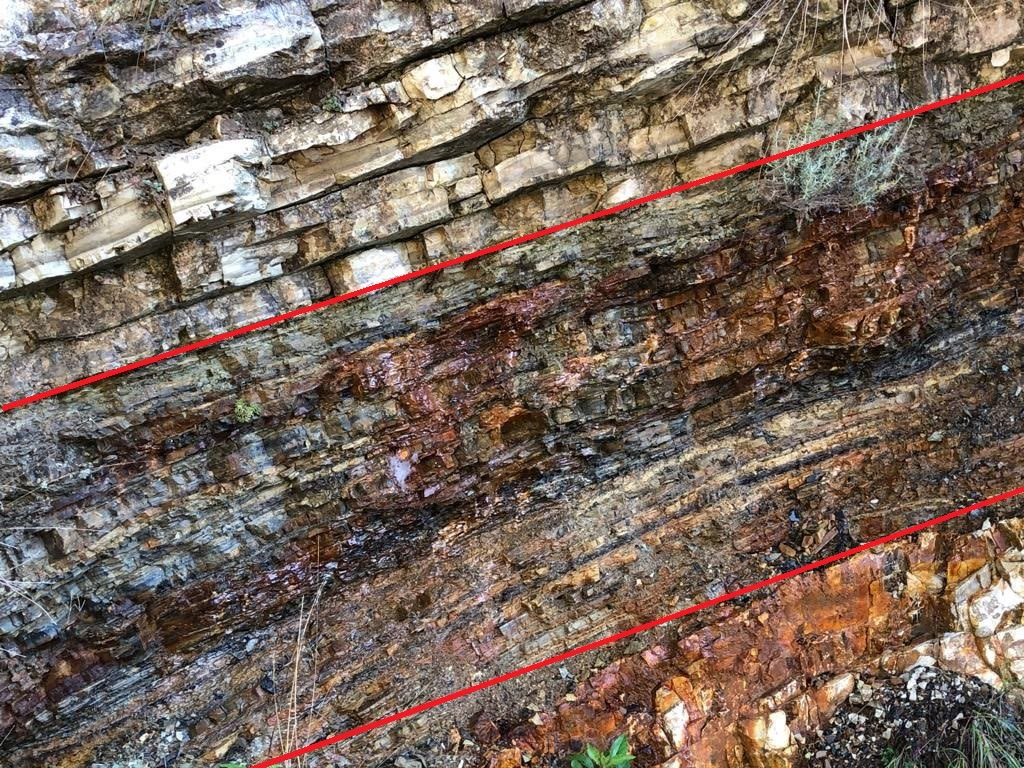
\includegraphics[width=0.66\linewidth]{images/book4/b2-19-bonarelli-level.jpg}
\par\smallskip{\small 博纳雷利层，即 OAE~2 的暗色页岩，夹于浅色石灰岩之间；
红线由摄影者所绘，标出其底界与顶界。（Picenus，CC~BY-SA~4.0，经
维基共享资源。）}
\end{omfigure}
% ledger: rigo24:oaes

\begin{inthefield}[记录一次缺氧事件]
一位研究远洋石灰岩剖面中 OAE 的地质学家逐层记录：层厚、
颜色、纹层、生物潜穴的有无、黄铁矿结核。她沿暗色层段采样，间隔紧密且规则，
并一直延伸到该层段之外很远，测定有机碳含量，以及有机物与碳酸盐的
碳同位素。同位素的偏移比岩石颜色更能把该事件从一个盆地关联到下一个盆地。
由于最暗的页岩可能出现在不同盆地的不同层位，
因此取同位素曲线而非黑色页岩，
作为时间标尺。
\end{inthefield}
% ledger: rigo24:oaes, wt24:oae2

\subsection*{希克苏鲁伯}

白垩纪末的灭绝有一个来自外部的成因。本科一年级分册讲过边界黏土中的铱
如何指向一次撞击，以及氩定年如何把该界线与希克苏鲁伯陨坑联系起来。
该构造直径约 \qty{200}{km}，年龄约 \qty{66}{Ma}；其
热岩石此后至少为循环水供热八百万年。对其地下不对称性的模型表明，撞击体来自东北方向，
与水平面成 45 至 \ang{60} 的夹角，
速度不低于地球逃逸速度 \qty{11.2}{km.s^{-1}}，更可能约为
\qty{20}{km.s^{-1}}。德干暗色岩在撞击前后同时正在喷发；
2010 年一篇对证据的综述认为，撞击触发了这次灭绝。
% ledger: pickersgill26:chicxulub, collins20:impact, renne:kpg, alvarez:iridium, schulte:kpg, cr03:deccan

\begin{dated}{2026}
本章年代采用《国际年代地层表》2026 年 6 月版，该版本为本系列各册通用；
海平面记录依其数据文件采用 2012 年的时间标尺，灭绝年代取自
Kaiho（2022）。该年代表随新测年数据的积累而修订，引用界线年代前，
请核对当前版本。
\end{dated}
% ledger: ics:base.Phanerozoic, data:b4-sealevel, kaiho22:table

\section*{练习}\label{sec:b2:phanerozoic-earth:exercises}

除非另有说明，练习数据如下：每度纬度 \qty{111.2}{km}；海底
深度 $d(t) = 2500 + 350\sqrt t$（\unit{m}，$t$ 以 \unit{Ma} 计）；海洋面积
\qty{362}{\mega km^2}；海底面积 \qty{293}{\mega km^2}；地幔密度
\qty{3300}{kg.m^{-3}}；海水 \qty{1025}{kg.m^{-3}}；大气质量
\qty{5.1e18}{kg}，空气与二氧化碳的摩尔质量分别为 \qty{28.97}{g.mol^{-1}} 和
\qty{44.01}{g.mol^{-1}}。
% ledger: earth:Rmean, ps77:depth-age, charette:ocean-volume, data:b4-ridge, katz03:thermo, noaa:seawater-1025, earth:Matm, earth:Mmol, ciaaw:abridged-2024

\begin{exercise}[$\star$]\label{exo:b2:phanerozoic-earth:1}
在地图模型中，\qty{300}{Ma} 前开普敦位于南纬 \ang{61.9}，纽约位于
南纬 \ang{3.6}；如今两地分别位于南纬 \ang{33.9} 和北纬 \ang{40.7}。（a）在四座城市中，哪一座
在 \qty{300}{Ma} 前位于赤道 \ang{30} 以内？（巴黎位于北纬 \ang{5.1}，悉尼位于
南纬 \ang{59.5}）？（b）开普敦与纽约自那时以来各自向北移动了多少千米？
（c）它们的平均速率各为多少，以厘米每年计？
\end{exercise}
% ledger: data:b4-palaeopos, geonames4:cities

\begin{exercise}[$\star$]\label{exo:b2:phanerozoic-earth:2}
五次大灭绝分别发生于 444、372、251.9、201.4 和 \qty{66}{Ma}。（a）求相继两次危机之间的间隔
及其平均值。（b）利用大火成岩省的平均年龄——
峨眉山 259、西伯利亚 250、CAMP 201、卡鲁–费勒 183、德干 \qty{65.5}{Ma}——五次危机中哪几次
落在某一大火成岩省的 \qty{2}{Ma} 之内？（c）平均间隔能否说明这些危机具有周期性？
\end{exercise}
% ledger: kaiho22:table, cr03:table

\begin{exercise}[$\star$]\label{exo:b2:phanerozoic-earth:3}
纪念碑岩的白垩约以每年 \qty{0.036}{mm} 的速率沉积。（a）
这 \qty{91}{m} 厚的白垩形成用了多长时间？（b）今天海面以每年 \qty{3.7}{mm} 上升，其速率是白垩沉积的多少倍？
（c）为什么海底能在不被泥掩埋的情况下，接收这样缓慢的沉积物？
\end{exercise}
% ledger: kgs:monument-rocks, ipcc:sea-level-obs

\begin{exercise}[$\star$]\label{exo:b2:phanerozoic-earth:4}
某悬崖自下而上依次为：带根痕的河流砂岩、含贝壳的海滩砂、灰色近岸
泥、白垩；白垩之上又覆有海滩砂。（a）该剖面在何处记录了
\omterm{def:b2:phanerozoic-earth:transgression}{海侵}，何处记录了\omterm{def:b2:phanerozoic-earth:transgression}{海退}？（b）\omterm{def:b2:phanerozoic-earth:transgression}{海侵}能否证明全球
海平面上升？（c）什么能使这一论证更有说服力？
\end{exercise}

\begin{exercise}[$\star\star$]\label{exo:b2:phanerozoic-earth:5}
在 Haq 等人的长期曲线上，海平面曾高出今日水平 \qty{233}{m}，
时刻为 \qty{97}{Ma}。（a）自那以来，平均下降速率为多少，
以米每百万年和微米每年表示？（b）与今天每年 \qty{3.7}{mm} 的上升相比。（c）经\omterm{def:b2:basins-compared:backstripping}{回剥}的
新泽西曲线在同一时刻约为 \qty{70}{m}。你更愿意相信哪条曲线给出的
振幅？为什么？
\end{exercise}
% ledger: data:b4-sealevel, ipcc:sea-level-obs, miller05:abstract, miller20:epr

\begin{exercise}[$\star\star$]\label{exo:b2:phanerozoic-earth:6}
CAMP 的单次脉冲，喷出约 \qty{e5}{km^3} 玄武岩，其密度为 \qty{2900}{kg.m^{-3}}，
喷发历时约 500 年。（a）若二氧化碳质量分数为 \qty{0.75}{\percent}，它释放了多少
千克，又合多少摩尔？（b）1750 年空气所含
二氧化碳的质量为多少（取 1750 年的 \qty{278}{ppm}）？（c）加以比较。（d）整个岩省
约 \qty{e5}{Gt}，能提供多少个这样的大气？
\end{exercise}
% ledger: capriolo20:camp-co2, ipcc:erf-2xco2, earth:Matm, earth:Mmol, ciaaw:abridged-2024

\begin{exercise}[$\star\star$]\label{exo:b2:phanerozoic-earth:7}
取希克苏鲁伯撞击体为直径 \qty{10}{km} 的球体，密度为
\qty{2630}{kg.m^{-3}}。（a）求其质量。（b）求其在最小可能速率
\qty{11.2}{km.s^{-1}} 与 \qty{20}{km.s^{-1}} 时的动能。（c）地球通过地表损失
内部热量为 \qty{47}{TW}，这些能量各相当于该热损失持续了多少年？
\end{exercise}
% ledger: alvarez:iridium, collins20:impact, b2dd10:half-space

\begin{exercise}[$\star\star$]\label{exo:b2:phanerozoic-earth:8}
（a）列出黑色页岩记录\omterm{def:b2:phanerozoic-earth:oae}{大洋缺氧事件}的特征。（b）将每一事件
与年龄相近的岩省配对：早托阿尔阶，\qty{183}{Ma}；OAE~1a，
\qty{120}{Ma}；已知卡鲁–费勒为 \qty{183}{Ma}，翁通爪哇为 \qty{122}{Ma}。（c）为何年龄相符
不足以证明某岩省引发了某一事件？
\end{exercise}
% ledger: rigo24:oaes, cr03:table

\begin{exercise}[$\star\star$]\label{exo:b2:phanerozoic-earth:9}
在该模型中，巴黎在 \qty{500}{Ma} 前位于南纬 \ang{60.9}，在 \qty{300}{Ma} 前位于北纬 \ang{5.1}。
（a）求其向北位移（分别以度和千米表示），并求平均速率，
以厘米每年计。（b）与 \qty{300}{Ma} 以来的速率相比
（见\cref{ex:b2:phanerozoic-earth:paris}）。（c）为何该速率为最小值？
\end{exercise}
% ledger: data:b4-palaeopos

\begin{exercise}[$\star\star\star$]\label{exo:b2:phanerozoic-earth:10}
设海底面积随年龄线性减小，从年龄 0 时的最大值
降至年龄 $T$ 时的零值。（a）证明平均年龄为 $T/3$，且 $\sqrt t$ 的平均值为
$\tfrac{8}{15}\sqrt T$。（b）若平均年龄为 \qty{64.2}{Ma}，求 $T$ 与平均深度。（c）
求扩张速率加倍时平均深度的下降量，并与
均匀模型中的 \qty{774}{m} 相比。（d）证明在两种模型中，下降量都接近 $0.93\,c\sqrt{\bar
t}\,(1 - f^{-1/2})$，其中 $\bar t$ 为平均年龄。
\end{exercise}

\begin{exercise}[$\star\star\star$]\label{exo:b2:phanerozoic-earth:11}
（a）由\cref{prop:b2:phanerozoic-earth:ridge}，证明 $\Delta s(f) = \Delta s(2)\,(1 -
f^{-1/2})/(1 - 2^{-1/2})$。（b）取 $\Delta s(2) = \qty{432}{m}$，求使
白垩纪峰值为 50 至 \qty{150}{m} 的 $f$ 的取值范围。（c）若扩张速率减慢至
今日的 0.8 倍会产生什么影响？（d）为什么由洋脊决定的长期海平面是一种缓慢的信号，
无论速率如何变化？
\end{exercise}
% ledger: data:b4-ridge, miller05:abstract

\begin{exercise}[$\star\star\star$]\label{exo:b2:phanerozoic-earth:12}
设物种以恒定速率灭绝，使同期群体中经过时间
$t$ 后仍存活的比例为 $2^{-t/m}$，物种寿命中位数 $m = \qty{2}{Ma}$。（a）
经过 \qty{7.4}{Ma}（即 1982 年分析的平均阶长）后，同期群中已消失的比例为多少？（b）
背景灭绝需要多长时间才能清除 \qty{81}{\percent} 的物种？（c）二叠纪末的
危机持续了约 \qty{60}{ka}，快了多少？（d）为什么粗略的时间
分辨率会模糊大灭绝与背景灭绝之间的差别？
\end{exercise}
% ledger: marshall23:resolution, stanley16:permian, burgess:end-permian

\begin{problem}[{周末问题——当洋脊扩张变快时}]\label{pb:b2:phanerozoic-earth:1}
本题要求计算：若洋脊扩张速度加倍，海平面将上升多少，
又将淹没多少陆地。取练习中的数据，洋底平均年龄为
\qty{64.2}{Ma}，洋脊全长 \qty{65000}{km}，今日海洋的水体积为
\qty{1.33e9}{km^3}，陆地面积为 \qty{148}{\mega km^2}。表中给出
今日陆地中海拔低于 $h$ 的百分比，数据取自一度网格的 ETOPO1。
\begin{center}
\small
\begin{tabular}{lcccccc}
\hline
$h$ (\unit{m}) & 0 & 100 & 200 & 300 & 400 & 500 \\
低于 $h$ 的陆地比例 (\unit{\percent}) & 0 & 14.9 & 28.2 & 38.7 & 48.1 & 55.8 \\
\hline
\end{tabular}
\end{center}
仿照\cref{prop:b2:phanerozoic-earth:ridge}，假设介于 0 与
洋底被俯冲时的年龄 $\tau$ 之间，每一个年龄的洋底所覆盖的面积都相同。

\noindent\textbf{第一部分——今日的洋底。}
\begin{enumerate}
  \item 求洋底在年龄 0、25、64.2 和 \qty{100}{Ma} 处的深度。
  \item 由平均年龄求 $\tau$，并求最老洋底的深度。
  \item 求平均全扩张速率 $u = A_{\text{f}}/(L\tau)$，单位为千米每
        百万年，并换算为毫米每年。它属于慢速、中速还是快速？
  \item 证明洋底的平均深度为 $2500 + \tfrac23 \times 350\sqrt\tau$，并
        计算其数值。
  \item 已测得有年代数据的洋底平均深度为 \qty{4265}{m}。试给出两条理由，说明
        为何模型给出的深度更大。
  \item 模型中，洋底之上的水体积为多少？与
        整个海洋的体积相比较。
\end{enumerate}

\noindent\textbf{第二部分——洋脊的剖面。}
\begin{enumerate}[resume]
  \item 求半扩张速率 $v$，精确到 \qty{0.1}{km.Ma^{-1}}，并求
        洋脊每一侧洋底的宽度。
  \item 距洋脊轴 \qty{1000}{km} 处的洋底深度为多少？
  \item 证明：洋脊在最老洋底深度以上的剖面，计入两侧
        后的面积为 $\tfrac23 v c\,\tau^{3/2}$，并计算其值，
        单位为平方千米。
  \item 求该深度以上整个洋脊系统的体积。
  \item 这一体积占海洋体积的多少？
  \item 为什么扩张较快的洋脊平均而言地势更高？
\end{enumerate}

\noindent\textbf{第三部分——速度加倍。}
\begin{enumerate}[resume]
  \item 扩张速率加倍，而洋底面积与洋脊长度保持不变。求新的 $\tau$
        和新的平均深度。
  \item 平均深度下降了多少？
  \item 洋底将多少体积的水挤出了盆地？
  \item 若将这部分水均匀分布于今日海洋上，海平面将上升多少？
  \item 计入洋底在多出的水重下的下沉，求上升量 $\Delta s$。
  \item 白垩纪的长期海平面峰值约为 \qty{100}{m}。扩张速率需增加多少，
        才能得到该数值？
\end{enumerate}

\noindent\textbf{第四部分——海水漫过陆地。}
\begin{enumerate}[resume]
  \item 海平面上升 \qty{100}{m}，将淹没多大面积的陆地？
  \item 海平面上升 \qty{432}{m} 时将淹没多大面积？用表中数据内插求出。
  \item 海水漫上陆地之后，为什么海平面的上升幅度必定小于 \qty{432}{m}？
  \item 以 \qty{100}{m} 为间隔，求海平面逐级抬升至 \qty{400}{m} 所需的体积，
        每一级上取被淹没面积的平均值（见\cref{prop:b2:phanerozoic-earth:flooding}）。
        需放置的体积为 $\qty{0.432}{km} \times \qty{362}{\mega km^2}$。海平面在何处
        停止上升？
  \item 此时海水覆盖了今日陆地的百分之几？
  \item 总结：在该模型中，扩张速率加倍将使海平面上升多少？
\end{enumerate}
\end{problem}
% ledger: ps77:depth-age, seton:mean-age, seton:rate-classes, noaa:ridge, charette:ocean-volume, data:b4-ridge, data:b4-floor-depth, katz03:thermo, noaa:seawater-1025, data:b4-hyps, miller05:abstract
